\documentclass[10pt]{article}
\usepackage[utf8]{inputenc}
\usepackage[activeacute,spanish]{babel}
\usepackage[left=1.5cm,top=1.5cm,right=1.5cm, bottom=1.5cm,letterpaper, includeheadfoot]{geometry}

\usepackage{amssymb, amsmath, amsthm}
\usepackage{graphicx}
\usepackage{hyperref}
\usepackage{lmodern,url}
\usepackage{paralist} %util para listas compactas
\usepackage{xcolor}
\usepackage{bbm}
\usepackage{mathrsfs}
\usepackage{bbm}

%========PAQUETES AGREGADOS===========
%Pseudocodigo
\usepackage{pseudocode}
\usepackage[portuguese, boxruled]{algorithm2e}
\usepackage{wrapfig}
\usepackage{multicol}
\usepackage{graphicx}
\usepackage{caption}
\usepackage{subcaption}
%\captionsetup[table]{labelformat=empty}
\captionsetup[subfigure]{labelformat=empty}
\usepackage{cancel}
\usepackage{tikz}
\def\checkmark{\tikz\fill[scale=0.4](0,.35) -- (.25,0) -- (1,.7) -- (.25,.15) -- cycle;} 
%====================================

\usepackage{fancyhdr}
\pagestyle{fancy}
\fancypagestyle{plain}{%
\fancyhf{}
\lhead{\footnotesize\itshape\bfseries\rightmark}
\rhead{\footnotesize\itshape\bfseries\leftmark}
}


% macros
\newcommand{\Q}{\mathbb Q}
\newcommand{\R}{\mathbb R}
\newcommand{\N}{\mathbb N}
\newcommand{\Z}{\mathbb Z}
\newcommand{\C}{\mathbb C}
\newcommand{\BigO}{\mathcal{O}}
%Teoremas, Lemas, etc.
\theoremstyle{plain}
\newtheorem{teo}{Teorema}
\newtheorem{lem}{Lema}
\newtheorem{prop}{Proposición}
\newtheorem{cor}{Corolario}
\newtheorem{obs}{Observación}
\newtheorem{ej}{Ejemplo}
\renewcommand{\qedsymbol}{\rule{0.7em}{0.7em}}
\renewenvironment{proof}{{\bfseries \noindent Demostración}}{ \qed \\}


\theoremstyle{definition}
\newtheorem{defi}{Definición}
% fin macros


\newcommand{\catnum}{15} %numero de catedra
\newcommand{\fecha}{13 de Septiembre 2016 }

%%%%%%%%%%%%%%%%%%

%Macros para este documento
\newcommand{\cin}{\operatorname{cint}}



\begin{document}
%Encabezado
\fancyhead[L]{Facultad de Ciencias Físicas y Matemáticas}
\fancyhead[R]{Universidad de Chile}
\vspace*{-1.2 cm}
\begin{minipage}{0.6\textwidth}
\begin{flushleft}
\hspace*{-0.5cm}\textbf{MA3402-1 Estadística. Primavera 2016}\\
\hspace*{-0.5cm}\textbf{Profesor:} Raul Gouet\\
\hspace*{-0.5cm}\textbf{Escriba:} Manuel Cáceres\\
\hspace*{-0.5cm}\textbf{Fecha:} \fecha
\end{flushleft}
\end{minipage}
\begin{minipage}{0.36\textwidth}
\begin{flushright}

\includegraphics[scale=0.3]{imagenes/fcfm_dcc}
\end{flushright}
\end{minipage}
\bigskip
%Fin encabezado

\begin{center}
\LARGE\textbf{Clase \catnum}
\end{center}
...Continuemos con los cálculos Bayesianos.\\

Retomamos el ejercicio con Bernoulli y a priori uniforme.\\

Tenemos una MAS $X_{1},\ldots,X_{n}$ del modelo de Bernoulli, cuya densidad (discreta) es 
\begin{align*}
f(X|\theta) = \theta^{\sum X_{i}}(1-\theta)^{n-\sum X_{i}}\\
X\in \{0,1\}^n, \theta \in \Theta = [0,1]
\end{align*}
Supongamos que $\pi(\theta)$ es la densidad Beta de parámetros $a,b>0$, es decir
\begin{align*}
\pi(\theta) &= \frac{\theta^{a-1}(1-\theta)^{b-1}}{Be(a,b)}\\
Be(a,b) &= \frac{\Gamma(a)\Gamma(b)}{\Gamma(a+b)}
\end{align*}
\textbf{NOTA:} Los parámetros de $\pi(\theta)$ (si hay) se llaman hiperparámetro, en este caso $a,b$.\\

Calculemos la densidad a posteriori de $\theta$, es decir, $\pi(\theta|X)$ (sería $f(\theta|X)$ pero usamos $\pi$ por tradición)
\begin{align*}
\pi(\theta|X) = \frac{f(X|\theta)\pi(\theta)}{f(X)} \alpha f(X|\theta)\pi(\theta)\\
\pi(\theta|X) \alpha \theta^{\sum X_{i}}(1-\theta)^{n-\sum X_{i}} \theta^{a-1}(1\theta)^{b-1}
\end{align*}
Recordemos que se trata de la densidad Beta de parámetros $\sum X_{i}+a$ y $n-\sum X_{i} +b$
\begin{align*}
\pi(\theta|X) = \frac{\theta^{\sum X_{i}+a-1}(1-\theta)^{n-\sum X_{i} +b -1}}{Be(\sum X_{i}+a,n-\sum X_{i}+b}
\end{align*}
En el caso de $\pi(\theta)$ uniforme (a=b=1), tenemos
\begin{align*}
\pi(\theta|X) = Beta(\sum X_{1} + 1, n-\sum X_{i}+1)
\end{align*}
\underline{Cálculo de la esperanza a posteriori:}
\begin{align*}
\mathbb{E}(\theta|X) = \int_{\Theta}\theta\pi(\theta|X)d\theta
\end{align*}
Si existe.\\
Aquí
\begin{align*}
&= \int_{0}^{1} \frac{\theta\theta^{\sum X_{i}+a-1}(1-\theta)^{n-\sum X_{i} +b - 1}}{Be(\sum X_{i}+a,n-\sum X_{i}+b)}d\theta\\
&= \int_{0}^{1}\frac{\theta^{\sum X_{i} +a}(1-\theta)^{n-\sum X_{i} + b -1}}{Be(\sum X_{i}+a,n-\sum X_{i}+b)}d\theta\\
&= \frac{Be(\sum X_{i} +a +1,n-\sum X_{i} +b)}{Be(\sum X_{i}+a, n-\sum X_{i} +b)}\\
&= \frac{(\sum X_{i}+a)\Gamma(\sum X_{i} + a)\Gamma(n-\sum X_{i} +b)}{(n+a+b)\Gamma(n+a+b)\Gamma(\sum X_{i}+a)\Gamma(n-\sum X_{i} + b)}\\
&= \frac{n\bar{X}+a}{n+a+b}
\end{align*}
Caso a=b=1, $\hat{\theta}_{B} := \mathbb{E}(\theta|X) = \frac{n\bar{X}+1}{n+2} \not = \bar{X}$, es decir, el estimador de Bayes es diferenctes al EIVUM de la tería clásica.\\

$\hat{\theta}_{B}$ es un resumen de $\pi(\theta|X)$ pero hay otras formas de proceder, si nos obligan a producir un estimador de $\theta$. Por ejemplo, la mediana a posteriori se calcula como:\\
$M$ tal que $\int_{0}^{M}\pi(\theta|X)d\theta = 1/2$.\\
Más popular que lo anterior es la moda. La moda de una densidad (o probabilidad) es el punto (no necesariamente único) donde se alcanza el máximo.
\begin{center}
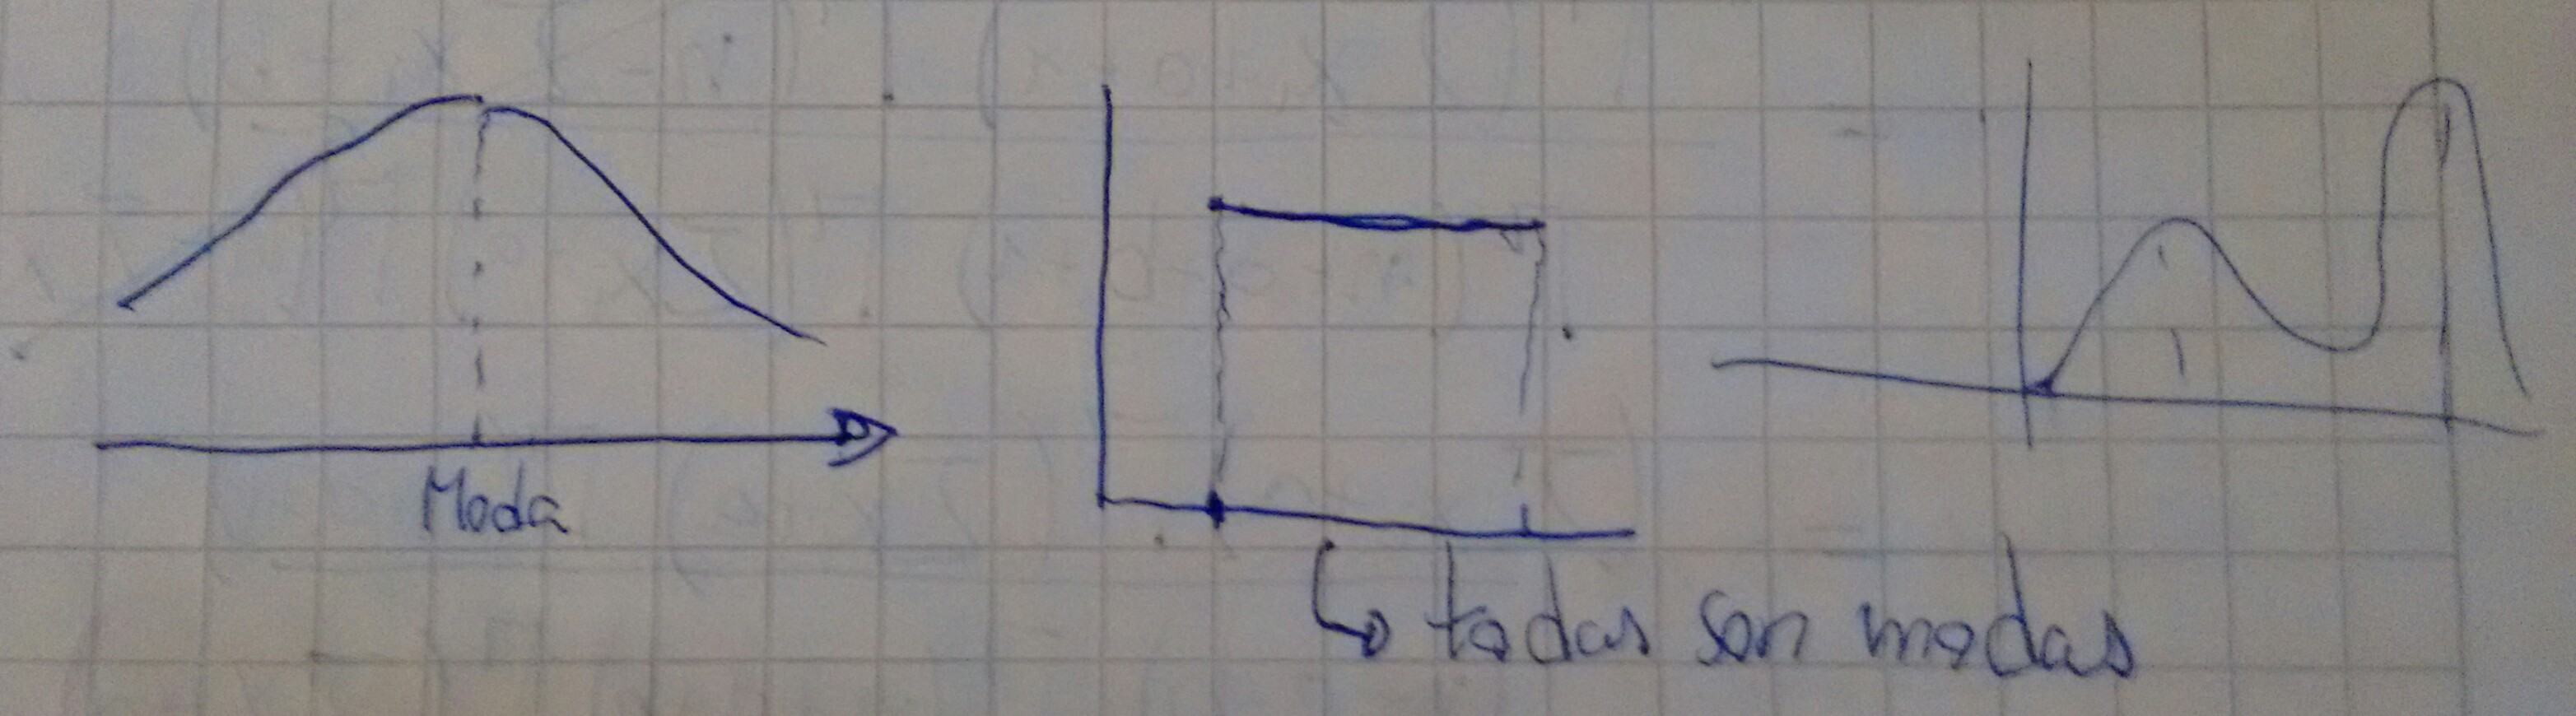
\includegraphics[scale=0.1]{imagenes/moda.jpg}
\end{center}
El estimador de $\theta$, llamado máximo a posteriori, denotado $\theta_{MAP}$ se calcula como
\begin{align*}
argmax_{\theta \in \Theta}\pi(\theta|X) & \text{ (es la moda)}
\end{align*}
Aquí en nuestro ejemplo tenemos
\begin{align*}
\pi(\theta|X) \sim \theta^{\sum X_{i} + \bar{a} - 1}(1-\theta)^{n-\sum X_{i} + \bar{b} - 1}\\
\max \theta^{\bar{a}-1}(1-\theta)^{\bar{b}-1}\\
\log \rightarrow (\bar{a}-1)\log \theta + (\bar{b}-1)\log (1-\theta)\\
\frac{\partial \log}{\partial \theta} \ldots \rightarrow \hat{\theta}_{MAP} = \ldots
\end{align*}
\textbf{¿Cómo se estima ``bayesianamente'' una función $g(\theta)$ de $\theta$?}\\
Lo que parece lógico es obtener la densidad a posteriori de $g(\theta)$, mediante cambio de variable.\\
Digamos que resulta $\pi_{g}(\tau|X), \tau = g(\theta)$ y calculamos $\hat{g}(\theta)_{B} = \mathbb{E}(g(\theta)|X)$.\\
Notar que no se necesita calcular $\pi_{g}(\tau|X)$ para obtener $\mathbb{E}(g(\theta|X)$. Basta escribir
\begin{align*}
\mathbb{E}(g(\theta)|X) = \int_{\Theta}g(\theta) \pi(\theta|X)d\theta
\end{align*}
\section{Conjugación}
Hemos visto en el ejemplo anterior ue $\pi(\theta)$ en Beta y que $\pi(\theta|X)$ también, con otros parámetros.\\

En este caso se habla de conjugación.\\
Dados $f(X|\theta)$ y $\pi(\theta)$ perteneciente a una familia, digamos $\mathcal{F}$, de densiddes sobre $\Theta$, diremos que hay conjugación, o que $\pi(\theta)$ es conjugada para $f(X|\theta)$, si $\pi(\theta|X) \in \mathcal{F}$.\\

Para que este concepto sea útil, hay que escoger $\mathcal{F}$ de forma que dependa de algunos pocos parámetros.\\

Porque en tal caso, el cálculo de $\pi(\theta|X)$ se reduce a una actualización de parámetros.\\

En nuestro ejemplo anterior $\mathcal{F} = \text{densidades Beta con parámetros a,b>0} = \{X^{a-1})(1-X)^{b-1}\colon a,b>0\}$, entonces $\pi(\theta) = Be(a,b) \in \mathcal{F}$ y $\pi(\theta|X) = Be(\sum X_{i} +a, n- \sum X_{i}+b) \in \mathcal{F}$.\\

Se produce una actualización de parámetros $a\sim \sum X_{i}+a, b \sim n-\sum X_{i}+b$.\\

Otro ejemplo interesante es el de las Poisson.
\begin{ej}
Sean $X_{1},\ldots,X_{n}$ iid. Poisson de parámetro $\theta>0$. Es decir,
\begin{align*}
f(X|\theta) = \frac{e^{-n\theta}\theta^{\sum X_{i}}}{\prod_{i=1}^{n}X_{i}!}\\
X_{i} \in \{0,1,\ldots\}, X = (X_{1},\ldots,X_{n}), \theta \in \Theta = (0,\infty)
\end{align*}
Vamos a tomar $\pi(\theta)$ como densidad gamma de parámetros $\lambda, p$ (hiperparámetros)
\begin{align*}
\pi(\theta) = \frac{\lambda (\lambda\theta)^{p-1}e^{-\lambda\theta}}{\Gamma(p)}\\
\lambda>0, p>0
\end{align*}
De lo anterior
\begin{align*}
\pi(\theta|X) &\alpha \frac{e^{-n\theta}\theta^{\sum X_{i}}}{\prod_{i=1}^n X_{i}!} \frac{\lambda (\lambda\theta)^{p-1}e^{-\lambda\theta}}{\Gamma(p)}\\
&\alpha e^{-\theta(\lambda+n)}\theta^{\sum X_{i}+p-1}
\end{align*}
Veremos que lo anterior es una densidad gamma de parámetro $\lambda+n,\sum X_{i} + p$.\\
\begin{align*}
\Rightarrow \pi(\theta|X) = \frac{(\lambda+n)((\lambda+n)\theta)^{\sum X_{i} + p - 1}e^{-(\lambda+n)\theta}}{\Gamma(p+\sum X_{i})}
\end{align*}
Esto revela que el modelo Poisson y la familia de densidades gamma, están en conjugación.
\end{ej}
Terminamos con otro ejemplo clásico de conjugación.
\begin{ej}
Sea $X_{1},\ldots,X_{n}$ MAS del modelo gaussiano $N(\theta,\sigma^2)$, donde $\sigma$ es conocido y $\theta$ parámetro real.\\
Consideremos $\pi(\theta)$ gaussiana $N(\mu,\tau^2)$, $\mu,\tau$ son hiperparámetros. Se calcula como:
\begin{align*}
\pi(\theta|X) &\alpha \underbrace{e^{-\frac{1}{2\sigma^2}\sum (X_{i}-\theta)^{2}}}_{f(X|\theta)}\underbrace{e^{-\frac{1}{2\tau^2}(\theta-\mu)^2}}_{\frac{\mu \theta}{\tau^2}}\\
&= e^{Q(\theta)} = N(\hat{\theta}(X),\hat{\sigma}^2(X))
\end{align*}
Hay que expandir las formas cuadráticas y agrupar convenientemente
\begin{align*}
Q &= -\frac{1}{2}\theta^2\left(\frac{n}{\sigma^2}+\frac{1}{\tau^2}\right) + \theta \left(\frac{\mu}{\tau^2}+\frac{n\bar{X}}{\sigma^2}\right) + \underbrace{R(x)}_{resto}\\
&= \ldots
\end{align*}
\end{ej}
\end{document}